\section{Bahasan Model Pemilihan}

\lettrine[nindent=-0.01em,findent=0.2em]{P}{ada} bagian ini, masing-masing pemodelan akan dijelaskan secara bertahap mulai dari pemodelan voting hingga pemodelan pemilihan yang disertai agen bayaran dengan SOP.

\subsection{Pemodelan Voting}

Model pemilihan dengan voting, menjadi inspirasi awal dalam pengembangan ini. Sebagai gambaran, pemilih ditentukan di awal adalah jumlah pemilih warna hijau.

\begin{equation}
	InitialGreenVoter = CountPatches \times \frac{InitialGreen}{100}
\end{equation}

\texttt{InitialGreenVoter} dapat dikatakan merepresentasikan estimasi dari jumlah keberpihakan suatu kelompok di lingkungan dan jumlah tick menggambarkan waktu yang menunjukkan bagaimana perkembangan keberpihakan dari setiap patch menurut waktu seperti Gambar \ref{fig:initvoter} berikut.

\begin{figure}[H]
	\centering
	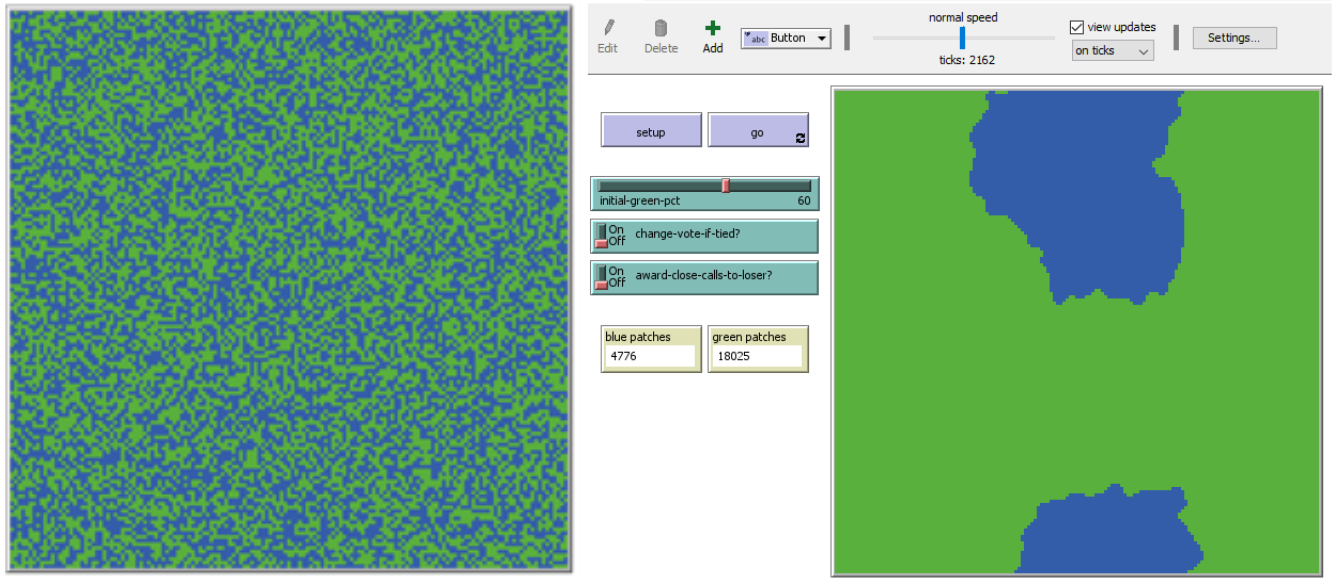
\includegraphics[width=\linewidth]{images/ch03/InitVoter}
	\caption{Simulasi voting NetLogo}
	\label{fig:initvoter}
\end{figure}

Pada model awal, jumlah initial patch hijau menentukan, artinya bila suatu kelompok sudah memiliki kecenderungan, kemungkinan komunitas akan mengikuti. Pada gambar di bawah, proporsi hijau diatur 50\% di awal, berkat ada interaksi antar agen jumlah akhir pemenangnya adalah biru dengan selisih yang tidak terlalu besar.

\begin{figure}[H]
	\centering
	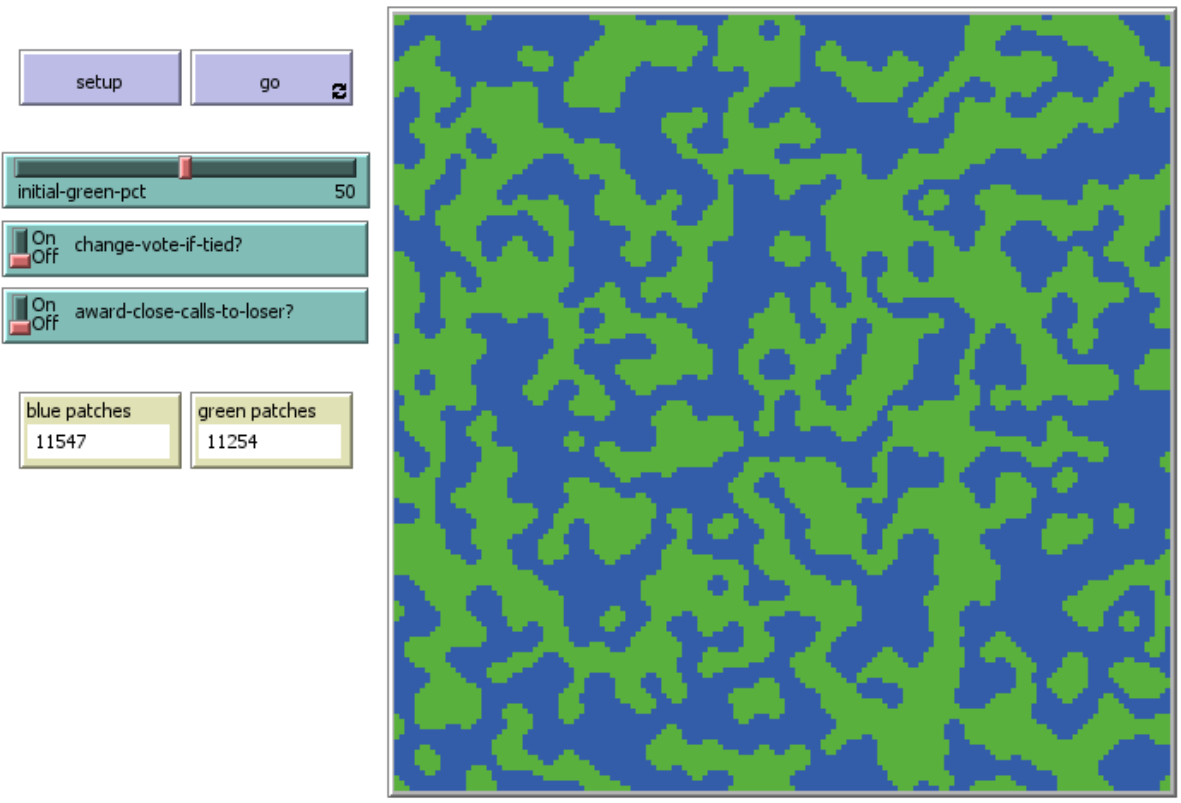
\includegraphics[width=\linewidth]{images/ch03/Voter2}
	\caption{Interaksi antar agen pemilih}
	\label{fig:voter2}
\end{figure}

\textbf{Change vote if tied}. Aturan default dari model ini adalah bila neighbours menunjukkan jumlah opini seri, maka sel akan tetap pada pilihan terakhir dan tidak berubah lagi seterusnya.

Opsi ini dapat merubah rule: bila seri, maka sel akan berubah. Hal ini membuat ketidakstabilan  dalam system yang menghasilkan noisy pada kesetimbangan. Hasilnya para agen tidak akan pernah berhenti bahkan saat sudah mencapai kestabilan global. Meski demikian, secara umum opsi ini tidak akan merubah skor dari distribusi opini, tetapi akan mengakibatkan beberapa agen merubah opini mereka secara terus menurus pada konfigurasi ini. Hasil simulasi pada modifikasi ini dapat dilihat dalam Gambar \ref{fig:voter3}.

\begin{figure}[H]
	\centering
	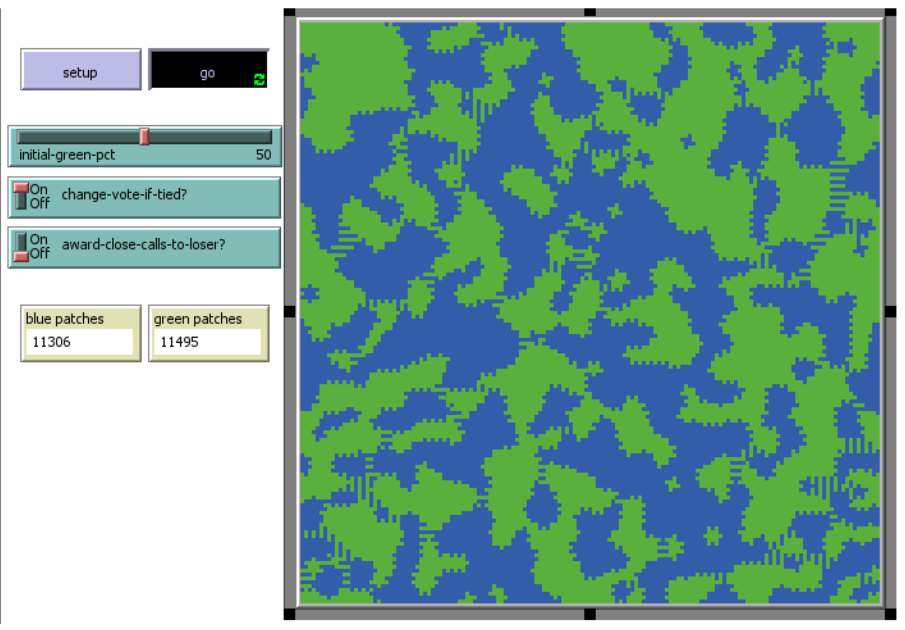
\includegraphics[width=\linewidth]{images/ch03/Voter3}
	\caption{Perubahan konfigurasi untuk pemilihan seri}
	\label{fig:voter3}
\end{figure}

\textbf{Award close calls to loser}. Konfigurasi dasar model ini adalah agen akan selalu mengikuti pilihan dari mayoritas dari agen-agen disekitarnya. Opsi ini meminta agen untuk memilih posisi minoritas secara sistemik. Dengan ini, hasil dari pemilihan bisa diluar ekspektasi. Dapat dibayangkan suatu society yang dipenuhi oleh agen-agen kontradiktif yang secara constant selalu berusaha merubah hasil. Lalu saat kesetimbangan sulit tercapai, dan minority tidak dapat mengubah pilihannya, system akan terus-menerus berubah menjadi satu warna dengan beberapa gelembung minoritas yang kecil didalamnya lalu menghadirkan ketidakstabilan yang tinggi.

Namun, untuk memperoleh hasil konstan seperti ini memerlukan waktu yang cukup lama. Kedua jenis agen ini dapat hidup bersama dalam jangka waktu yang cukup lama. Terkadang kelas yang kalah kembali menyamakan kedudukan dengan yang menang, terkadang dia terus berisolaso antara 8000-9000 melawan mayoritas 13000-12000.

Hal yang dapat dipahami dari Gambar \ref{fig:voter4} adalah bahwa dalam komunitas masyarakat demokrasi, hasil pemungutan suara pada saat-saat tertentu dapat berubah dan tidak terduga dan tidak dapat dikatakan menjadi dasar sebagai perkiraan hasil pada pemungutan suara yang lain.

\begin{figure}[H]
	\centering
	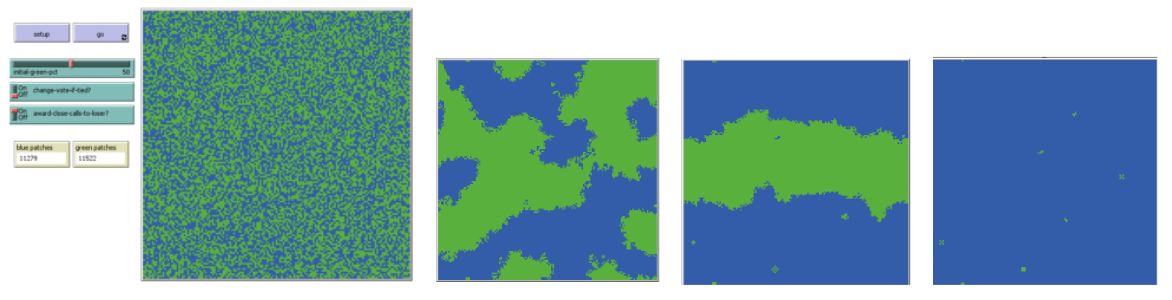
\includegraphics[width=\linewidth]{images/ch03/Voter4}
	\caption{Perubahan bertahap selama voting}
	\label{fig:voter4}
\end{figure}

Setelah 90.000 iterasi model masih belum mencapai titik kesetimbangan. Walaupun dapat diramalkan bahwa model akan berakhir dimenangkan oleh patch biru dan terdapat beberapa titik-titik hijau.

Pada konsep pemilihan umum dengan pemilih bayaran yang akan dikembangkan, para agen netral akan digiring oleh agen-agen bayaran yang ditempatkan untuk membuat pilihan mengikuti pilihan dari agen bayaran. Bagaimana perilaku dari agen dapat terpengaruh oleh agen lain, dapat dilihat pada bagian model standing ovation berikut.

\subsection{Pemodelan SOP di NetLogo}

Untuk model SOP dengan lima tetangga dapat dilakukan dengan menggunakan model kerucut dengan panjang barisan 1. Pada kasus selanjutnya misalkan untuk $L=20$ (terdapat 20 baris penonton), maka model kerucut dapat diimplementasikan hingga $n=18$.


\subsubsection{Skenario lima tetangga - synchronous updating}

Lima tetangga dengan nilai $cone-length=1$, $noise=0$, $intrinsic-proc-standing=0.42$, $updating=synchronous updating$ dan pengaturan yang dipilih \texttt{Make guy stand up}. Berikut akan diperlihatkan apa yang dilihat oleh agen.

\begin{figure}[H]
	\centering
	\subfloat[Kondisi awal]{
		\label{sfig:sop1}
		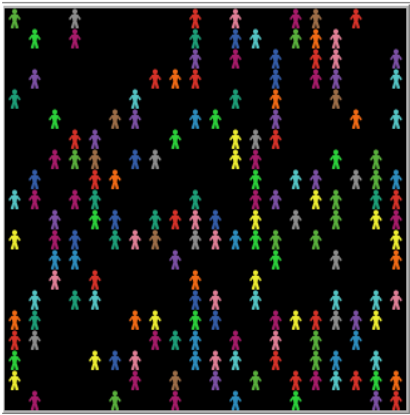
\includegraphics[width=0.3\linewidth]{images/ch03/sop1}
	}\hfill
	\subfloat[Saat $t=1$]{
		\label{sfig:sop2}
		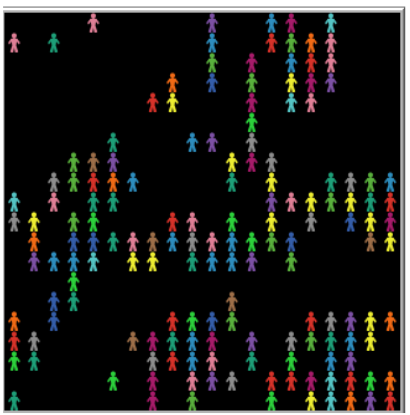
\includegraphics[width=0.3\linewidth]{images/ch03/sop2}
	}\hfill
	\subfloat[Saat $t=10$]{
		\label{sfig:sop3}
		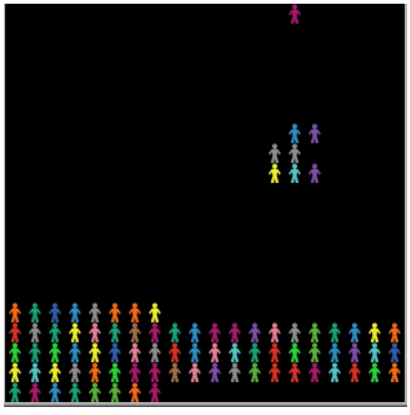
\includegraphics[width=0.3\linewidth]{images/ch03/sop3}
	}\hfill
	\caption{Proses iterasi standing ovation di NetLogo}
	\label{fig:proses_sop}
\end{figure}

Pada saat $t=27$ diperoleh dengan tidak ada seorangpun yang berdiri dengan $t$ menyatakan jumlah iterasi. Pada model ini, setiap agen bergerak mengikuti perubahan yang terjadi di sekitarnya.

\begin{figure}[H]
\centering
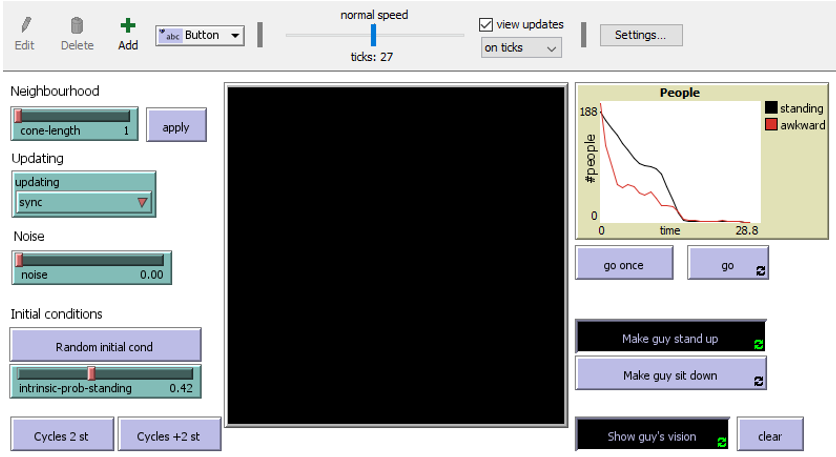
\includegraphics[width=\linewidth]{images/ch03/sop4}
\caption{Hasil simulasi saat $t=27$}
\label{fig:sop4}
\end{figure}

\subsubsection{Skenario lima tetangga - asynchronous updating}

Lima tetangga dengan nilai $cone-length=1$, $noise=0$, $intrinsic-proc-standing=0.42$, $updating=asynchronous updating$ dan pengaturan yang dipilih \texttt{Make guy stand up}. Berikut akan diperlihatkan apa yang dilihat oleh agen.

\begin{figure}[H]
	\centering
	\subfloat[Kondisi awal]{
		\label{sfig:sop4}
		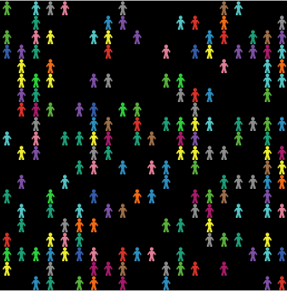
\includegraphics[width=0.3\linewidth]{images/ch03/sop5}
	}\hfill
	\subfloat[Saat $t=1$]{
		\label{sfig:sop5}
		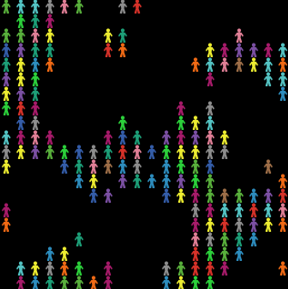
\includegraphics[width=0.3\linewidth]{images/ch03/sop6}
	}\hfill
	\subfloat[Saat $t=10$]{
		\label{sfig:sop6}
		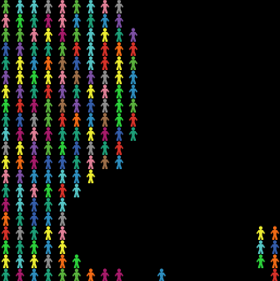
\includegraphics[width=0.3\linewidth]{images/ch03/sop7}
	}\hfill
	\caption{Proses iterasi standing ovation asynchronous updating di NetLogo}
	\label{fig:proses_sop_async}
\end{figure}

Pada skenario ini di iterasi $t=36$ agen masih belum konvergen dikarenakan agen secara random memperhatikan sekitarnya. Bisa dikatakan pada situasi ini seolah penonton terbagi di dua kelompok.

\begin{figure}[H]
\centering
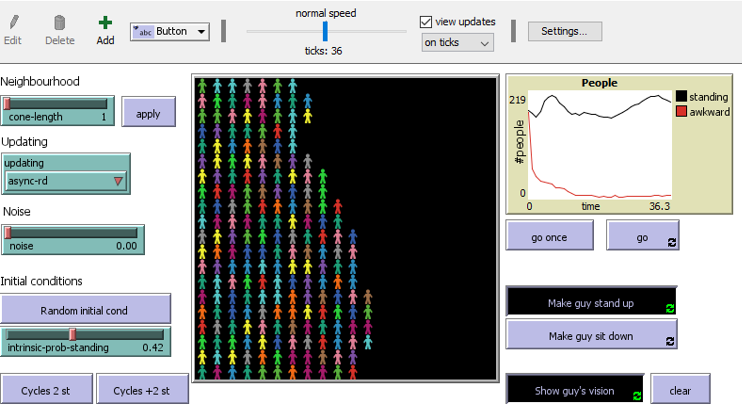
\includegraphics[width=\linewidth]{images/ch03/sop8}
\caption{Hasil simulasi saat $t=36$}
\label{fig:sop8}
\end{figure}

\subsubsection{Skenario Lingkungan kerucut - synchronous updating}

Kerucut dengan nilai $cone-length=18$, $noise=0.5$, $intrinsic-proc-standing=0.5$, $updating= synchronous updating$ dan pengaturan yang dipilih \texttt{Make guy stand up}. Berikut akan diperlihatkan apa yang dilihat oleh agen.

\begin{figure}[H]
	\centering
	\subfloat[Kondisi awal]{
		\label{sfig:sop7}
		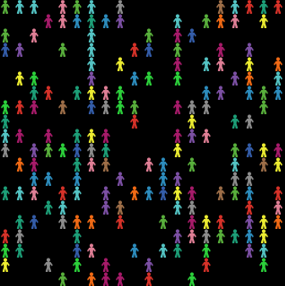
\includegraphics[width=0.3\linewidth]{images/ch03/sop9}
	}\hfill
	\subfloat[Saat $t=1$]{
		\label{sfig:sop8}
		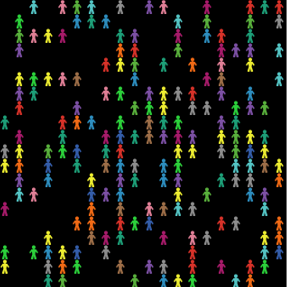
\includegraphics[width=0.3\linewidth]{images/ch03/sop10}
	}\hfill
	\subfloat[Saat $t=10$]{
		\label{sfig:sop9}
		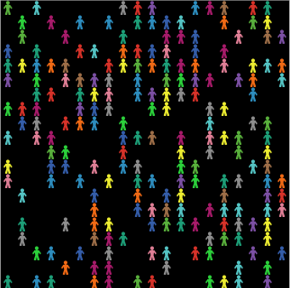
\includegraphics[width=0.3\linewidth]{images/ch03/sop11}
	}\hfill
	\caption{Proses iterasi standing ovation kerucut synchronous updating di NetLogo}
	\label{fig:proses_sop_kerucut_sync}
\end{figure}

Pada skenario ini, di iterasi $t=36$ agen masih belum konvergen dikarenakan pada kerucut jumlah pengaruh yang diterima setiap agen lebih tinggi. Pada perubahan setiap agen pada tiap waktu secara bersamaan, perubahan akan lebih mudah terprediksi karena sangat bergantung terhadap kondisi awal. Pada skenario 2, noise diaktifkan untuk memberikan perubahan dinamik pada model lebih signifikan. Noise juga membantu agar sistem tidak terkunci pada suatu state.

\begin{figure}[H]
\centering
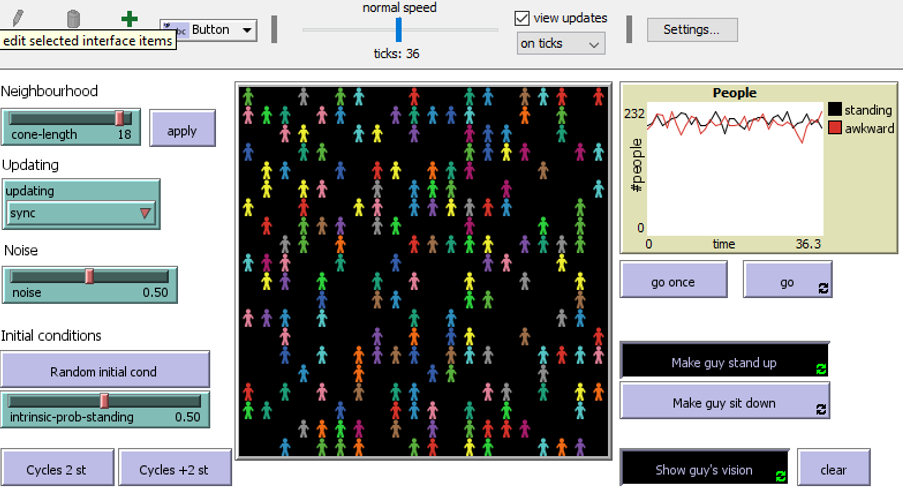
\includegraphics[width=\linewidth]{images/ch03/sop12}
\caption{Hasil simulasi saat $t=36$}
\label{fig:sop12}
\end{figure}

\subsubsection{Skenario Lingkungan kerucut - asynchronous updating}

Kerucut dengan nilai $cone-length=18$, $noise=0.5$, $intrinsic-proc-standing=0.5$, $updating=synchronous updating$ dan pengaturan yang dipilih \texttt{Make guy stand up}. Berikut akan diperlihatkan apa yang dilihat oleh agen.

\begin{figure}[H]
	\centering
	\subfloat[Kondisi awal]{
		\label{sfig:sop10}
		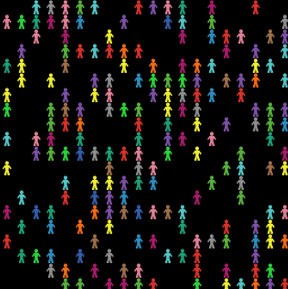
\includegraphics[width=0.3\linewidth]{images/ch03/sop13}
	}\hfill
	\subfloat[Saat $t=1$]{
		\label{sfig:sop11}
		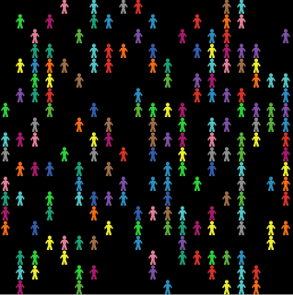
\includegraphics[width=0.3\linewidth]{images/ch03/sop14}
	}\hfill
	\subfloat[Saat $t=10$]{
		\label{sfig:sop12}
		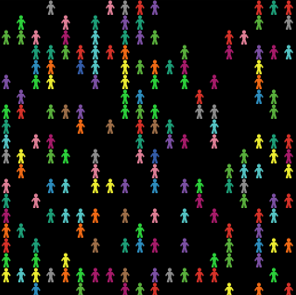
\includegraphics[width=0.3\linewidth]{images/ch03/sop15}
	}\hfill
	\caption{Proses iterasi standing ovation kerucut asynchronous updating di NetLogo}
	\label{fig:proses_sop_kerucut_async}
\end{figure}

Pada skenario ini, di iterasi $t=36$ agen masih belum konvergen dikarenakan pada kerucut jumlah pengaruh yang diterima setiap agen lebih tinggi. Karena setiap agen berubah secara random pada waktu yang berbeda. Maka, terdapat keterkaitan yang lebih rumit. Perubahan pada agen di baris $n+1$ tergantung pada perubahan agen di baris $n$.

\begin{figure}[H]
\centering
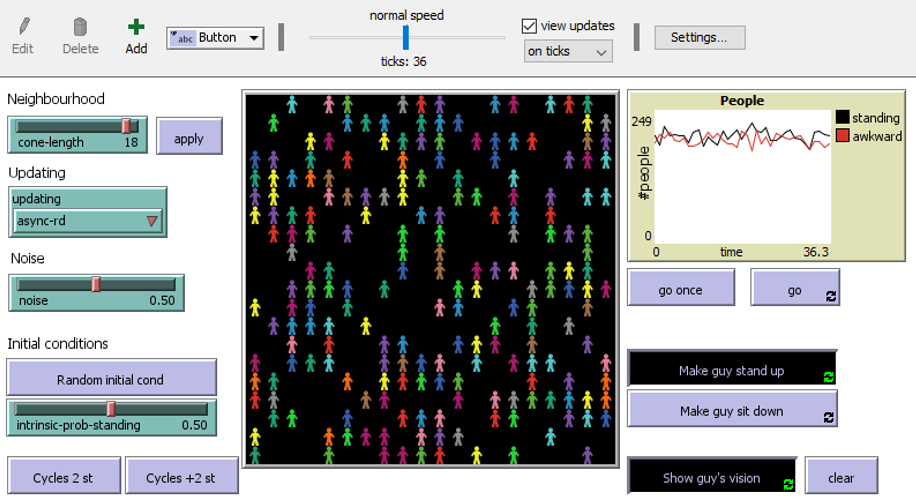
\includegraphics[width=\linewidth]{images/ch03/sop16}
\caption{Hasil simulasi saat $t=36$}
\label{fig:sop13}
\end{figure}

Dalam kaitannya dengan pemilih bayaran, model standing ovation dapat dijadikan rujukan untuk menunjukkan bahwa individu dapat merubah keputusannya akibat ada perubahan di sekelilingnya dan noises memberikan state lebih dinamis.

\subsection{Model Pemilihan dengan SOP di NetLogo}

Berdasarkan Algoritma \ref{alg:sop_sederhana} dapat diterapkan di \texttt{NetLogo} dengan tampilan seperti Gambar \ref{fig:pemilusop1} berikut ini:

\begin{figure}[H]
\centering
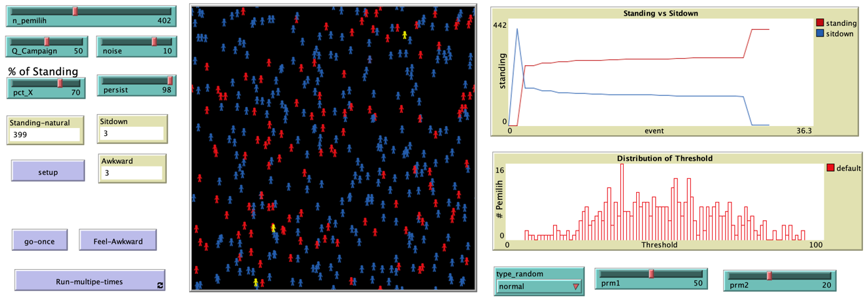
\includegraphics[width=\linewidth]{images/ch03/pemilusop1}
\caption{Implemetasi pemilihan umum dengan SOP di NetLogo}
\label{fig:pemilusop1}
\end{figure}

Dari Gambar \ref{fig:pemilusop1}, Beberapa variabel dapat dijelaskan sebagai berikut:

\begin{itemize}
\item $n\_pemilih$ digunakan untuk membuat banyaknya agen (pemilih)

\item $Q_{Campaign}$ digunakan untuk menentukan kualitas dari kampanye calon atau kandidat

\item $Noise$ digunakan untuk memberikan dinamika dari model yang dibuat dan mendekati kejadian sebenarnya

\item $pct\_X$ digunakan untuk menentukan batas ketidaknyamanan (\textit{awkward level}), apabila total pemilih yang berdiri lebih besar dari $pct\_X$ maka sisa pemilih akan ikut berdiri

\item $persist$ digunakan untuk menentukan batas threshold yang tidak terpengaruh dengan kondisi apapun.
\end{itemize}

Dengan menggunakan model sederhana, dapat melihat simulasi dengan berbagai kondisi misalnya:

\begin{itemize}
\item Bagaimana jika kualitas kampanye rata-rata (mediocre), dan penilaian pemilih juga rata-rata (mediocre)

\item Bagaimana pengaruh jika pemilih memiliki level ketidaknyamanan (awkward) tinggi atau rendah

\item Bagaimana pengaruh jika masyarakat pemilih sangat apatis, walau-pun kualitas kampanye bagus atau sebaliknya
\end{itemize}

\subsubsection{Skenario model sederhana 1}

Pada skenario 1, simulasi dilakukan dengan kondisi kampanye dari kandidat atau calon rata-rata (\textit{mediocre}) dan masyarakat pemilih memberikan penilaian biasa saja (\textit{mediocre}).

Untuk pemodelan ini, konfigurasi yang digunakan yaitu jumlah\\ $n\_pemilih=402$, $Q_{campaign}=50$, $noise=10$ dan distribusi \texttt{threshold uniform} dengan nilai 30 hingga 100.

\begin{figure}[H]
\centering
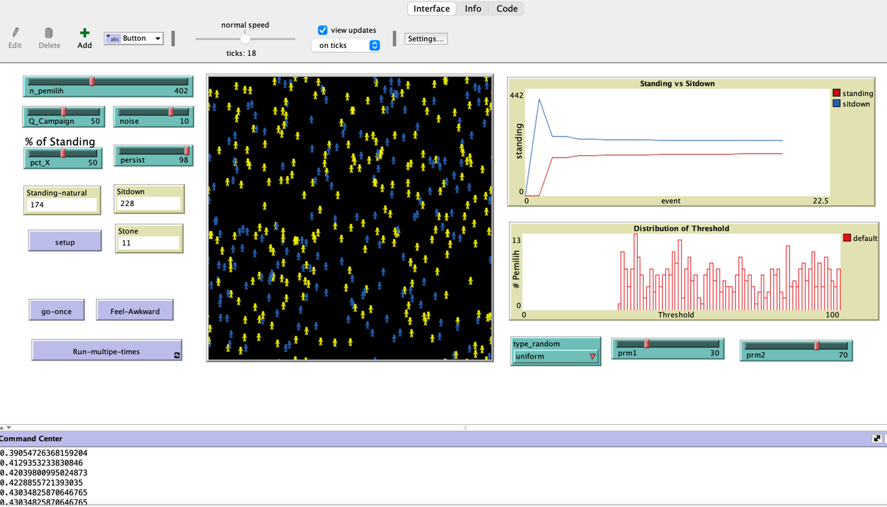
\includegraphics[width=\linewidth]{images/ch03/pemilusop2}
\caption{Konfigurasi skenario 1 pada pemilihan umum dengan SOP}
\label{fig:pemilusop2}
\end{figure}

Gambar \ref{fig:pemilusop2} diatas adalah hasil simulasi dengan parameter yang sudah ditentukan. Dari grafik Standing terhadap Sitdown, dapat dilihat bahwa pemilih pada tahap awal $40\%$ memutuskan untuk memilih dan secara bertahap naik sampai $43\%$, sedangkan sisanya tetap Sitdown atau tidak memilih. Pada siklus (iterasi) selanjutnya dikarenakan tidak ada faktor lain yang mempengaruhi, maka komposisi jumlah pemilih yang Standing (memilih) dan jumlah pemilih yang Sitdown (tidak memilih) tetap. Kita dapat memperhatikan pengaruh distribusi threshold pemilih dengan menggunakan tipe uniform akan menghasilkan pola pemilih yang berimbang.

Dalam skenario 1 ini, dapat dilakukan perubahan distribusi \textit{threshold} menggunakan tipe normal (\textit{Gaussian}) dengan mean (rata-rata) 51 dan standar deviasi (simpangan) 20. Hasil dari simulasi seperti Gambar \ref{fig:pemilusop3} dibawah ini.

\begin{figure}[H]
\centering
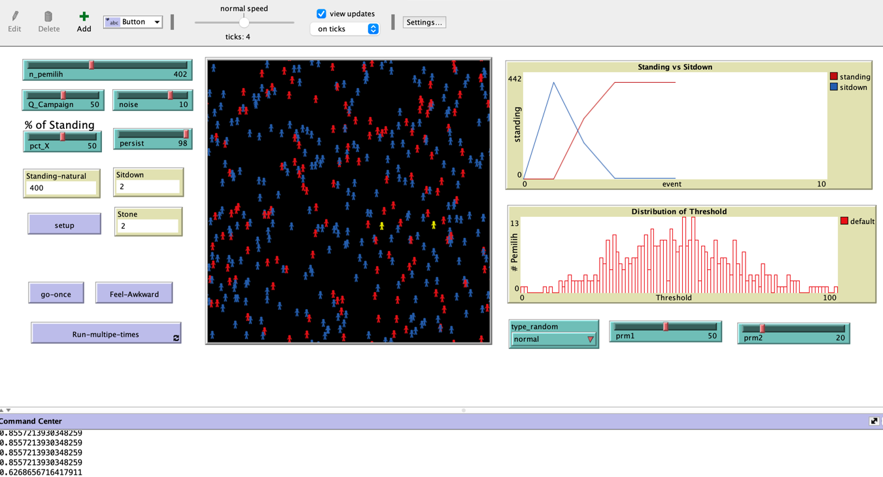
\includegraphics[width=\linewidth]{images/ch03/pemilusop3}
\caption{Perubahan konfigurasi jenis distribusi acak pada skenario 1}
\label{fig:pemilusop3}
\end{figure}

Dengan merubah tipe distrubis \textit{threshold}, setelah 2 kali iterasi, pemilih yang awalnya Sitdown (tidak memilih) berubah pikiran menjadi Standing (memilih), sehingga mayoritas Standing tercapai. Beberapa pemilih tetap pada pendirian awal, Sitdown, karena mempunyai threshold (99), masuk dalam kelompok \textit{Stoner} (orang orang yang keras kepala).

Tipe distribusi (sebaran) \textit{threshold} ini untuk memodelkan kondisi masya-rakat, untuk tipe masyarakat yang sangat heterogen, dapat menggunakan tipe uniform, akan tetapi untuk masyarakat yang homogen dan mempunyai kecenderungan tertentu (preferensi) kita bisa gunakan distribusi tipe Normal (\textit{Gaussian}), dengan standar deviasi makin kecil menandakan tingkat keseragaman (homogen) makin tinggi.

\subsubsection{Skenario model sederhana 2 dengan pengaruh ketidaknyamanan (\textit{awkward})}

Pada skenario ini, perubahan level ketidaknyamanan (\textit{awkward}) terhadap perilaku pemilih diterapkan. Skenario 2 menggunakan parameter yang dikembangkan dari skenario 1 dengan menurunkan $pct\_X$, semakin rendah nilainya maka orang akan semakin tidak nyaman dan berubah pilihannya dan ikut Standing (memilih). Parameter $pct\_X$ diturunkan menjadi 40 (persen) sehingga apabila jumlah pemilih yang Standing dibagi total pemilih dan melebihi $pct\_X$ maka sisa pemilih akan berubah ikut Standing (pemilih).

\begin{figure}[H]
\centering
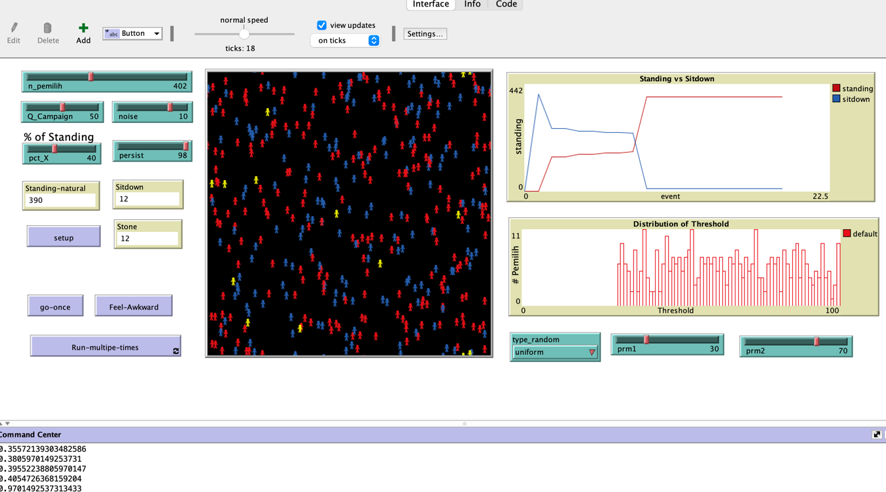
\includegraphics[width=\linewidth]{images/ch03/pemilusop4}
\caption{Pengaruh tingkat ketidaknyaman pemilih di pemilihan dengan SOP}
\label{fig:pemilusop4}
\end{figure}

Gambar \ref{fig:pemilusop4} diatas adalah hasil simulasi dengan menurunkan $pct\_X$ (awkward limit) dari $50\%$ menjadi $40\%$. Dengan perubahan parameter ini, setelah melalui 4 siklus iterasi, sebagian besar pemilih yang awalnya masih Sitdown (tidak memilih), akan berubah pikiran menjadi Standing (memilih) karena total pemilih yang berdiri dibagi jumlah pemilih sudah lebih besar dari $40\%$.

\subsubsection{Skenario model sederhana 3}

Pada skenario 3, simulasi pemilih yang apatis (berpikir apriori) terhadap kandidat atau calon dilakukan ketika kualitas kampanye biasa-biasa saja (\textit{mediocre}). Parameter yang akan digunakan dalam simulasi ini adalah $Q_{campaign}=50$, tipe distribusi \textit{threshold} Normal (\textit{Gaussian}) dengan rata-rata $60$ dan standar deviasi $10$ serta $pct\_X=50$. Hasil simulasi memberikan hasil sebagai berikut:

\begin{figure}[H]
\centering
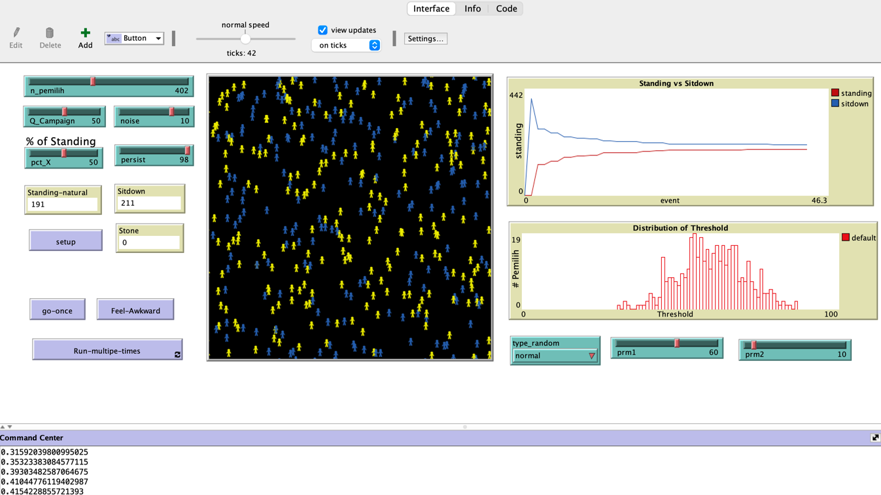
\includegraphics[width=\linewidth]{images/ch03/pemilusop5}
\caption{Perubahan konfigurasi untuk kualitas kampanye calon}
\label{fig:pemilusop5}
\end{figure}

Dari Gambar \ref{fig:pemilusop5} bagian grafik \textit{Standing vs Sitdown}, setelah 9 siklus (iterasi), jumlah pemilih yang menyatakan Standing (memilih) mencapai $47\%$ dari total pemilih dan tetap pada nilai tersebut pada iterasi selanjutnya dan seterusnya. Hal ini karena tidak ada lagi faktor yang mempengaruhi pemilih untuk berubah pikiran.

Apabila ingin mencapai level mayoritas pemilih Standing (memilih), maka harus menurunkan $pct\_X$ (batas ketidaknyamanan) menjadi $40$, hasil dari simulasi model akan menjadi sebagai berikut:

\begin{figure}[H]
\centering
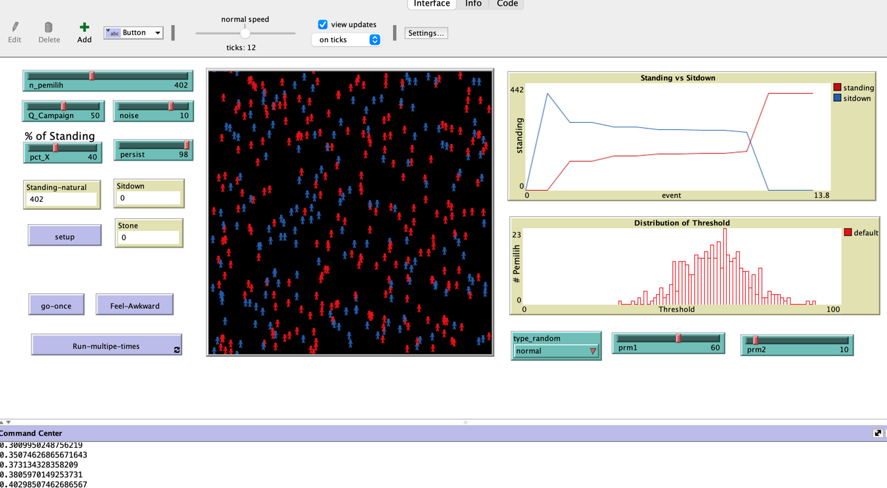
\includegraphics[width=\linewidth]{images/ch03/pemilusop6}
\caption{Perubahan sikap pemilih ketika tingkat ketidaknyamanan diturunkan}
\label{fig:pemilusop6}
\end{figure}

\subsubsection{Skenario model kompleks 1}

Pada bagian ini, skenario dilakukan dengan menggunakan model kompleks. Parameter yang digunakan adalah $n\_pemilih=402$, $Q_{campaign}=30$, $noise=10$, tipe distribusi Normal (\textit{Gaussian}) dengan $mean=50$ dan $std=10$, $n\_agen\_bayar=40$, $modal=0$ dan $money_pol=10$ (jumlah uang setiap pemberian). Dalam model awal ini, tidak ada uang yang dibagikan untuk pemilih. Model ini sebagai model acuan untuk melihat pengaruh pemberian uang oleh agen bayaran. Untuk lebih jelasnya, berikut ini merupakan konfigurasi parameter seperti Gambar \ref{fig:pemilusop7} dibawah ini:

\begin{figure}[H]
\centering
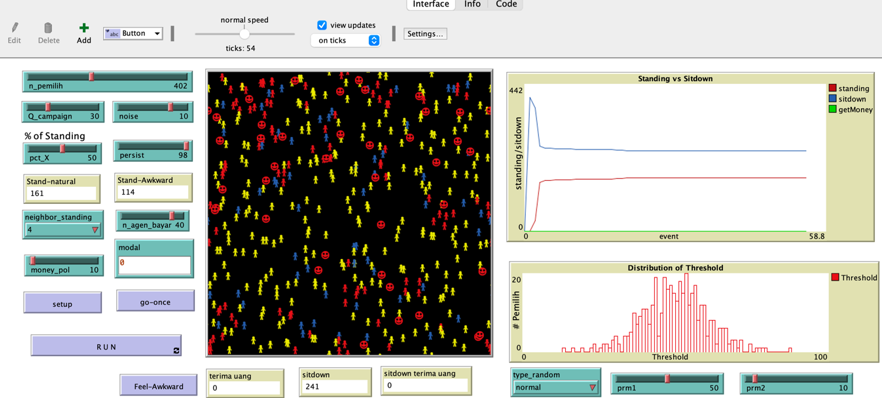
\includegraphics[width=\linewidth]{images/ch03/pemilusop7}
\caption{Konfigurasi parameter untuk model kompleks}
\label{fig:pemilusop7}
\end{figure}

Hasil simulasi menunjukan, jumlah pemilih yang Standing (memilih) sebanyak $161$, sementara yang Sitdown (tidak memilih) $241$. Kemudian dari skenario awal tersebut penambahan parameter modal, yaitu sejumlah uang yang akan dibagikan oleh $40$ agen bayaran kepada masing-masing pemilih sebesar $10$ dan akan mengurangi threshold pemilih sebesar $10$. Modal yang dimiliki oleh setiap $agen\_bayar=100$, dan hasil simulasi yang didapatkan adalah sebagai berikut:

\begin{figure}[H]
\centering
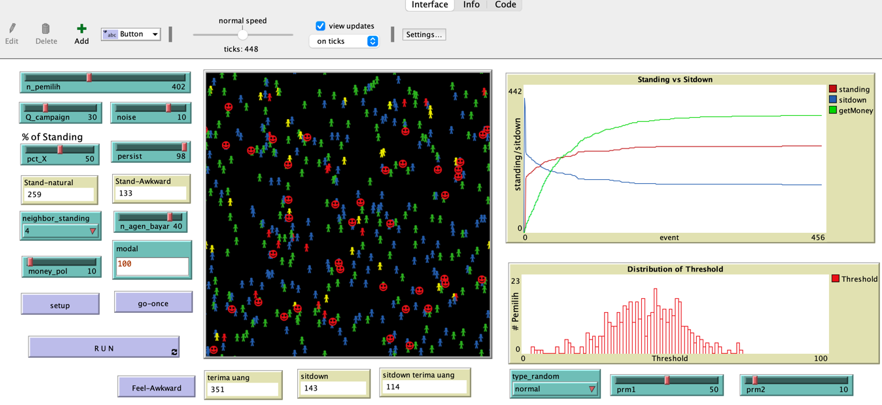
\includegraphics[width=\linewidth]{images/ch03/pemilusop8}
\caption{Perubahan beberapa konfigurasi dari parameter awal}
\label{fig:pemilusop8}
\end{figure}

Dari Gambar \ref{fig:pemilusop8} bagian grafik dapat diketahui bahwa jumlah pemilih yang Standing (memilih) sebanyak $259$ orang, sementara yang Sitdown $143$, jumlah pemilih yang Standing (memilih) lebih besar dari Sitdown (tidak memilih) dan hasil akhir dari distribusi \textit{threshold} dari pemilih juga berubah, angka \textit{mean} (rata-rata) bergeser ke kiri atau lebih rendah dari \textit{mean} sebelumnya $50$ atau dengan kata lain \textit{threshold} dari pemilih turun dikarenakan menerima uang.

Dari Gambar \ref{fig:pemilusop8} juga, jumlah pemilih yang menerima uang dan tetap Sitdown (tidak memilih) sebesar $114$ dan ditandai dengan agen berwarna hijau. Hal ini terjadi karena kualitas kampanye ($Q_{campaign}$) yang rendah.

Untuk meningkatkan jumlah pemilih Standing (memilih) dan mendapatkan hasil pemilih mayoritas diatas $80\%$ dengan kondisi kualitas kampanye $30$, kita dapat memperbesar pembagian uang ke pemilih menjadi $20$ dan modal yang dimiliki setiap $agen\_bayar=200$. Gambar berikut ini adalah hasil simulasinya:

\begin{figure}[H]
\centering
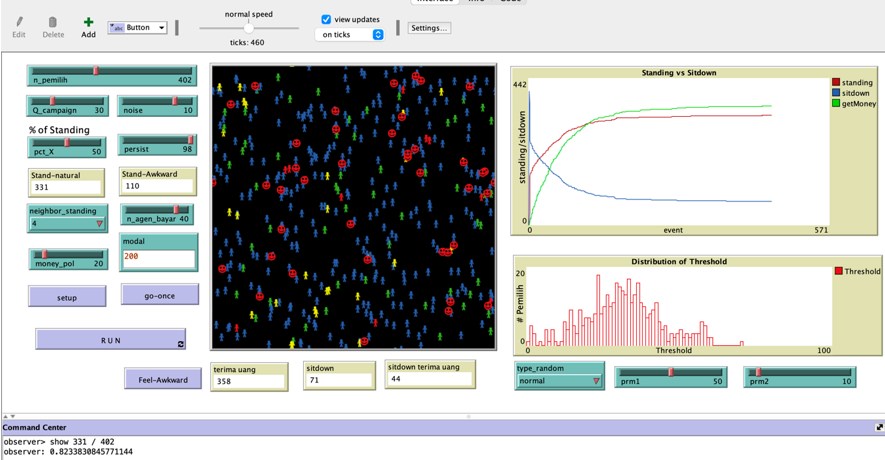
\includegraphics[width=\linewidth]{images/ch03/pemilusop9}
\caption{Konfigurasi parameter yang dilakukan agar pemilih mayoritas lebih dari $80\%$}
\label{fig:pemilusop9}
\end{figure}

Dari Gambar \ref{fig:pemilusop9}, Diperlukan $326$ siklus (iterasi) untuk mencapai jumlah pemilih Standing (memilih) sebesar $83\%$ dari total pemilih dan hanya $44$ orang pemilih yang mendapatkan uang, namun tidak berubah pilihannya. Dari total $331$ orang pemilih yang Standing (memilih), $110$ diantaranya Standing dikarena faktor pemilih sekitar (awkward). Dengan demikian,dapat ditarik kesimpulan bahwa pemberian uang oleh agen berpengaruh terhadap pilihan pemilih.

Bagaimana jika nilai uang yang dibagikan diperbesar dan jumlah modal tetap sama? Berikut ini adalah hasil simulasinya:

\begin{figure}[H]
\centering
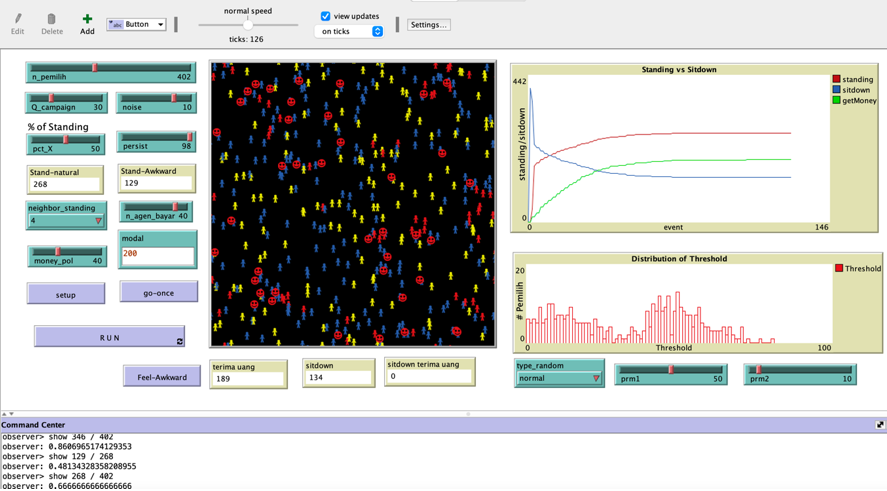
\includegraphics[width=\linewidth]{images/ch03/pemilusop10}
\caption{Pengaturan konfigurasi jumlah uang dinaikkan tapi modal tetap}
\label{fig:pemilusop10}
\end{figure}

Apabila dibandingkan hasilnya dengan simulasi sebelumnya, dengan menaikan nilai uang untuk pemilih dapat ditarik kesimpulan sebagai berikut:

\begin{enumerate}
\item Persentase pemilih yang Standing (memilih) karena terpengaruh pemilih sekitar lebih besar pada pembagian nominal yang lebih besar atau dengan kata lain

\item Persentase total pemilih yang Standing (memilih) terhadap total pemilih lebih besar pada pembagian nominal lebih kecil

\item Jika tujuannya untuk meraih suara pemilih terbanyak, pembagian dengan nominal lebih kecil lebih efektif untuk mendapatkan jumlah pemilih yang Standing (memilih)
\end{enumerate}

Untuk model kompleks yang sama, perubahan parameter dilakukan pada penambahan batas pemilih sebesar $8$ yang dapat menyebabkan seorang pemilih merubah pilihannya. Apabila pemodelan tersebut dijalankan untuk beberapa siklus (iterasi) akan didapatkan hasil sebagai berikut:

\begin{figure}[H]
\centering
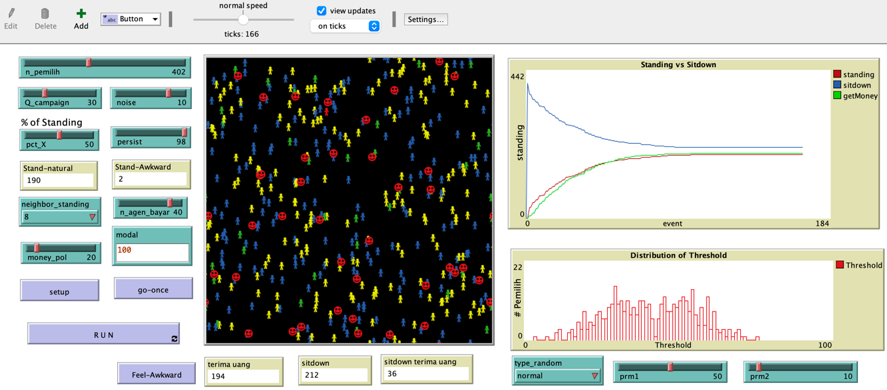
\includegraphics[width=\linewidth]{images/ch03/pemilusop11}
\caption{Perubahan simulasi akibat penambahan jumlah batasan pemilih}
\label{fig:pemilusop11}
\end{figure}

Dari hasil simulasi diatas, jumlah pemilih yang Standing (memilih) $190$ lebih kecil dibandingkan dengan pemilih yang Sitdown (tidak memilih) $212$. Setelah mencapai siklus (iterasi) $100$ dan komposisi pemilih yang Standing dan Sitdown tetap serta tidak ada faktor lain yang bisa mempengaruhi keputusan dikarenakan uang modal sudah terdistribusi ke semua pemilih. Jumlah pemilih yang Standing karena pemilih sekitar (\textit{awkward}) hanya dua orang.

Pada Gambar \ref{fig:pemilusop12} berikut, jumlah pemilih sekitar yang akan mempengaruhi keputusan diturunkan menjadi 4, artinya diperlukan 4 pemilih sekitar (tetangga) yang Standing untuk membuat seorang pemilih berubah menjadi Standing.

\begin{figure}[H]
\centering
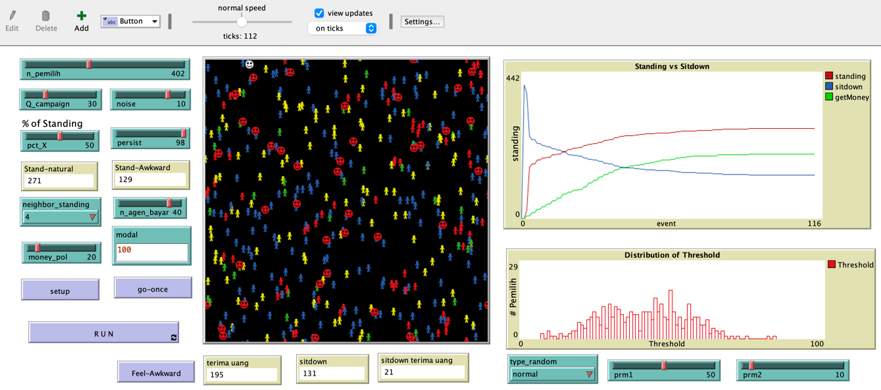
\includegraphics[width=\linewidth]{images/ch03/pemilusop12}
\caption{Penguragan jumlah tetangga sekitar yang dapat mempengaruhi pemilih}
\label{fig:pemilusop12}
\end{figure}

Dengan parameter seperti gambar diatas, jumlah pemilih yang Standing (memilih) akan meningkat dibandingkan dengan sebelumnya dan jumlah pemilih Standing $271$ lebih besar dibandingkan dengan pemilih Sitdown $195$. Pada sisi lain, terjadi penurunan jumlah pemilih terima uang yang tetap Sitdown (tidak memilih) $21$ dari sebelumnya $36$.

Perlu diketahui juga dari hasil simulasi ini, untuk masyarakat pemilih yang lebih mandiri (independen), dengan nilai $neighbor\_stand=8$, pengaruh pemberian uang tidak dapat membuat jumlah pemilih Standing (memilih) lebih besar dari pemilih yang Sitdown (tidak memilih).

\subsection{Model Pemilihan dengan SOP di Python Mesa}

Setelah memahami penggunaan Persamaan \ref{eq:sop_mesa} serta penjelasan ringkas terhadap Algoritma \ref{alg:modelagenbayaran}, \ref{alg:agenbayaran}, dan \ref{alg:agenpemilih} maka pemodelan pemilihan umum dengan SOP di ABM dapat dibuat ke dalam bentuk aplikasi berbasis web \cite{Zikri_Modified_Standing_Ovation_2021} dengan tampilan umum seperti Gambar \ref{fig:mesa0}. Ada beberapa skenario yang akan dilakukan, adapun penjelasannya sebagai berikut.

\begin{figure}[H]
\centering
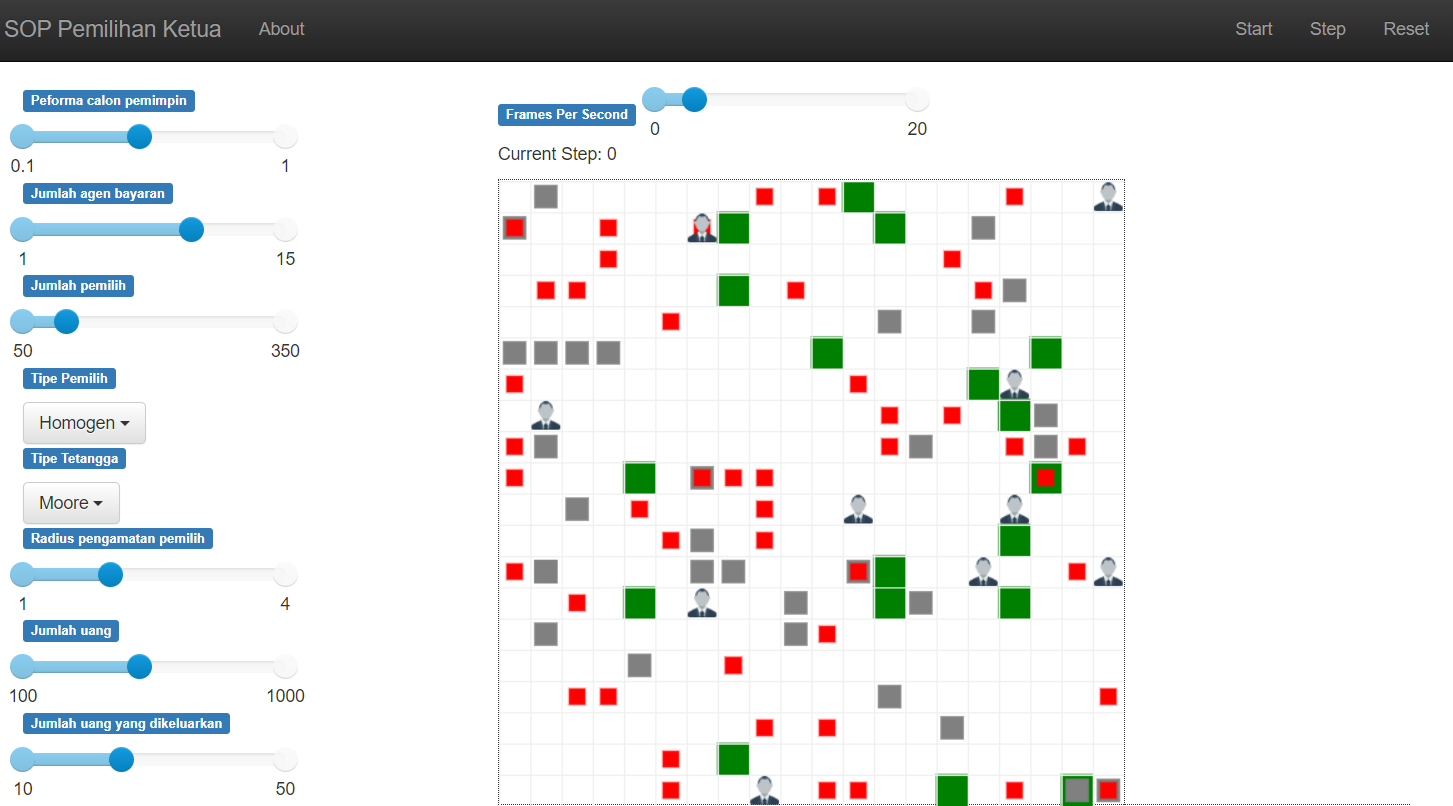
\includegraphics[width=\linewidth]{images/ch03/mesa0}
\caption{Aplikasi berbasis web dengan Python Mesa}
\label{fig:mesa0}
\end{figure}


\subsubsection{Skenario Pesimis}

Pada skenario ini konfigurasi \texttt{input} diatur seminimal mungkin. Hal ini dapat dilihat dalam Tabel \ref{tab:pengaturanpesimis} dibawah dengan $N_{ab}$ adalah jumlah agen bayaran, $N_{p}$ adalah jumlah pemilih, dan $R$ adalah radius pengamatan.

\begin{table}[H]
\centering
\caption{Pengaturan aplikasi untuk skenario pesimis}
	\begin{tabular}{cccccccc}
	\hline
	Peforma & $N_{ab}$ & $N_{p}$ & $Tipe_{pemilih}$ & $Tipe_{tetangga}$ & R & uang & keluar \\
	\hline
	0.1 & 1 & 50 & Heterogen & Von Neumann & 1 & 100 & 10\\
	\hline
	\end{tabular}
  \label{tab:pengaturanpesimis}
\end{table}

Dengan pengaturan diatas, didapatkan sebaran acak awal untuk masing-masing agen bayaran dan pemilih seperti Gambar \ref{fig:mesa1}. Perlu diketahui bahwa dalam aplikasi berbasis web ini memiliki beberapa simbol. Adapun penjelasan dari masing-masing simbol sebagai berikut.

\begin{table}[H]
\centering
\caption{Simbol-simbol dalam keseluruhan aplikasi}
	\begin{tabular}{cccc}
	\hline
	Avatar & Merah & Abu-abu & Hijau \\
	\hline
	Agen bayaran & Pemilih tidak milih & Pemilih ragu & Pemilih milih \\
	\hline
	\end{tabular}
  \label{tab:simbolaplikasi}
\end{table}

\begin{figure}[H]
\centering
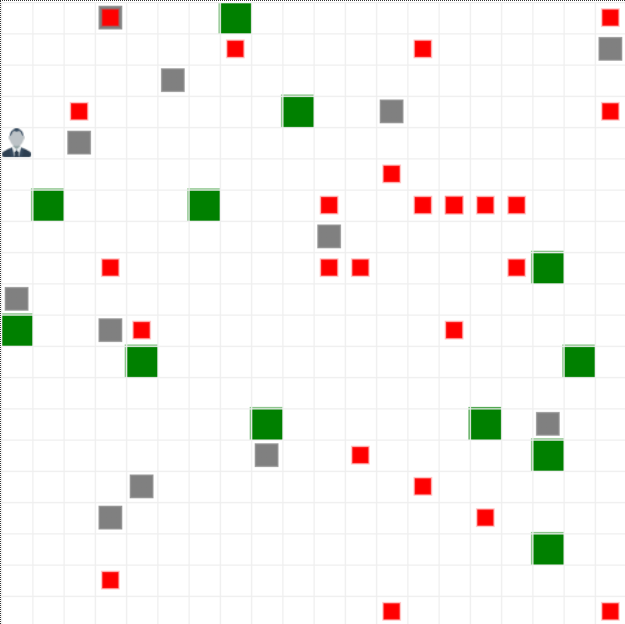
\includegraphics[width=0.8\linewidth]{images/ch03/mesa1}
\caption{Sebaran acak awal pada skenario pesimis}
\label{fig:mesa1}
\end{figure}

Apabila simulasi ini dijalankan selama 1065 iterasi, agen bayaran sudah meninggalkan tempat seperti Gambar \ref{sfig:mesa2} karena walaupun uang yang dikeluarkan sedikit sebesar 10 namun modal awal yang dipegang hanya 100. Dengan kata lain, agen bayaran hanya dapat memberikan uang 10 kali kepada agen pemilih.

\begin{figure}[H]
	\centering
	\subfloat[Agen bayaran tidak aktif]{
		\label{sfig:mesa2}
		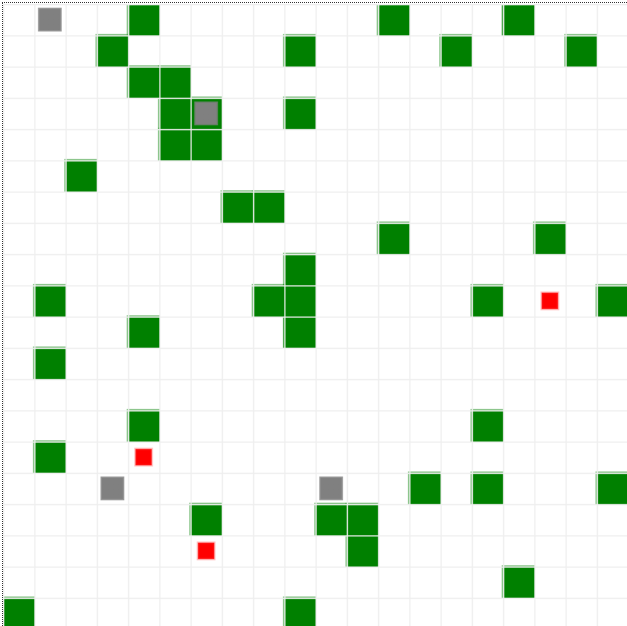
\includegraphics[width=0.48\linewidth]{images/ch03/mesa2}
	}\hfill
	\subfloat[Saat $t=1065$]{
		\label{sfig:mesa3}
		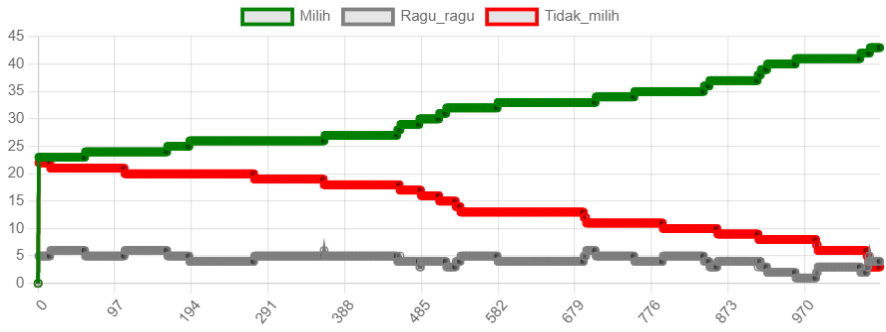
\includegraphics[width=0.48\linewidth]{images/ch03/mesa3}
	}\hfill
	\caption{Simulasi pemilihan di skenario pesimis}
	\label{fig:simulasi_mesa_pesimis}
\end{figure}

Berdasarkan Gambar \ref{sfig:mesa3}, perlu iterasi yang lama agar agen pemilih mulai terpengaruh untuk yakin memilih. Hal ini dapat disebabkan karena peforma calon pemimpin tidak bagus dan disertai konfigurasi lain yang minimum. Kondisi ini dapat terjadi di lapangan, namun hal menarik dapat terjadi di skenario pesimis ini yaitu dengan meningkatkan jarak radius pengamatan dari konsep SOP ini.

\begin{figure}[H]
	\centering
	\subfloat[Agen bayaran tidak aktif]{
		\label{sfig:mesa4}
		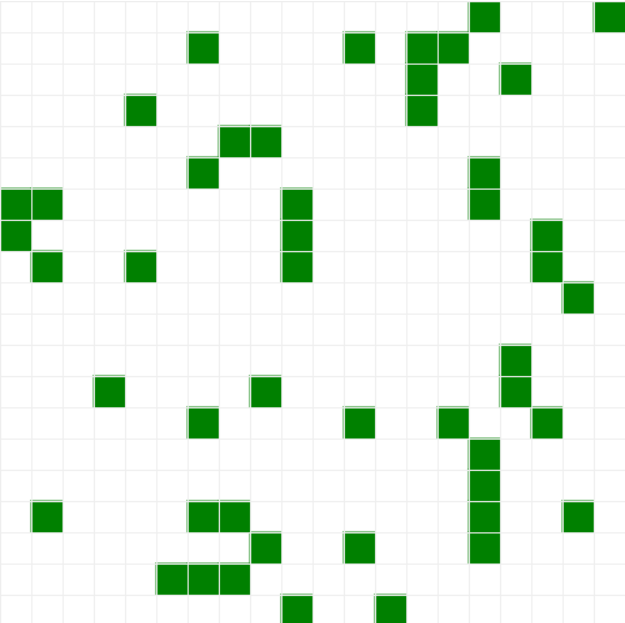
\includegraphics[width=0.48\linewidth]{images/ch03/mesa4}
	}\hfill
	\subfloat[Saat $t=124$]{
		\label{sfig:mesa5}
		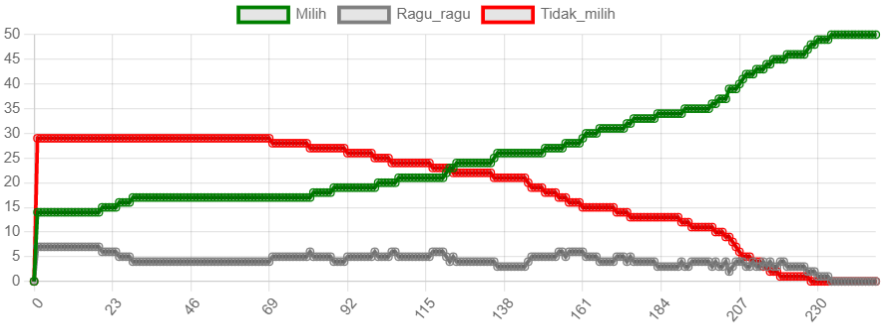
\includegraphics[width=0.48\linewidth]{images/ch03/mesa5}
	}\hfill
	\caption{Simulasi pemilihan di skenario pesimis dengan radius pengamatan}
	\label{fig:simulasi_mesa_pesimis_2}
\end{figure}

Tidak diragukan lagi dari Gambar \ref{sfig:mesa5}, agen pemilih semula tidak memilih atau ragu-ragu, lalu mulai meningkat keinginan untuk memilih walaupun sebenarnya peforma calon pemimpin tidak bagus dan agen bayaran sudah meninggalkan tempat seperti Gambar \ref{sfig:mesa4}. Hal inilah yang membuat skenario pesimis menjadi menarik karena efek dari radius pengamatan agen pemilih yang ditingkatkan menyebabkan pemberian pengaruh menjadi lebih besar. Perlu diketahui juga bahwa disini peforma calon pemimpin tidak baik bisa jadi cara menyampaikan atau komunikasi tidak tepat walaupun sebenarnya calon tersebut memiliki perilaku yang baik dan begitu pula sebaliknya bisa saja peforma baik saat kampanye namun perilaku asli dari calon tidak baik.

Yang patut menjadi pertanyaan adalah bagaimana meningkatkan radius pengamatan di lapangan dengan kondisi minimalis seperti Tabel \ref{tab:pengaturanpesimis}? Dengan meningkatnya penggunaan jejaring sosial, langkah yang dapat diambil dalam rangka agar agen pemilih mau menambahkan radius pengamatan adalah calon pemimpin juga giat dalam memanfaatkan fitur yang diberikan jejaring sosial karena fasilitas ini gratis dan cocok dengan pengeluran yang ketat.

Apabila trafik calon pemilih berhasil didapatkan maka fenomena baru muncul yaitu efek atau pengaruh dari interaksi antar agen pemilih (saling mempengaruhi) diharapkan dapat memberikan \textbf{sentimen positif} terhadap calon pemimpin. Dalam kondisi ini agen bayaran hanya memberikan stimulus awal selnajutnya agen bayaran meniggalkan sistem seperti Gambar \ref{sfig:mesa4} dan sisanya adalah saling mempengaruhi antar agen pemilih dalam jarak radius tertentu.

\subsubsection{Skenario Ideal}

Pada skenario ini konfigurasi \texttt{input} diatur seideal mungkin. Hal ini dapat dilihat dalam Tabel \ref{tab:pengaturanideal} dibawah. Peforma calon pemimpin dianggap "pas-pasan" dalam skenario ini dengan parameter lain disesuaikan.

\begin{table}[H]
\centering
\caption{Pengaturan aplikasi untuk skenario ideal}
\begin{tabular}{cccccccc}
	\hline
	Peforma & $N_{ab}$ & $N_{p}$ & $Tipe_{pemilih}$ & $Tipe_{tetangga}$ & R & uang & keluar \\
	\hline
	0.5 & 10 & 100 & Homogen & Moore & 2 & 500 & 25\\
	\hline
\end{tabular}
\label{tab:pengaturanideal}
\end{table}

Apabila simulasi ini dijalankan pada iterasi 84, agen pemilih mulai terpengaruh (Gambar \ref{sfig:mesa7}) untuk memilih dan agen bayaran masih aktif melakukan tebar pengaruh ke calon pemilih lainnya seperti Gambar \ref{sfig:mesa6} berikut.

\begin{figure}[H]
	\centering
	\subfloat[Agen bayaran masih aktif]{
		\label{sfig:mesa6}
		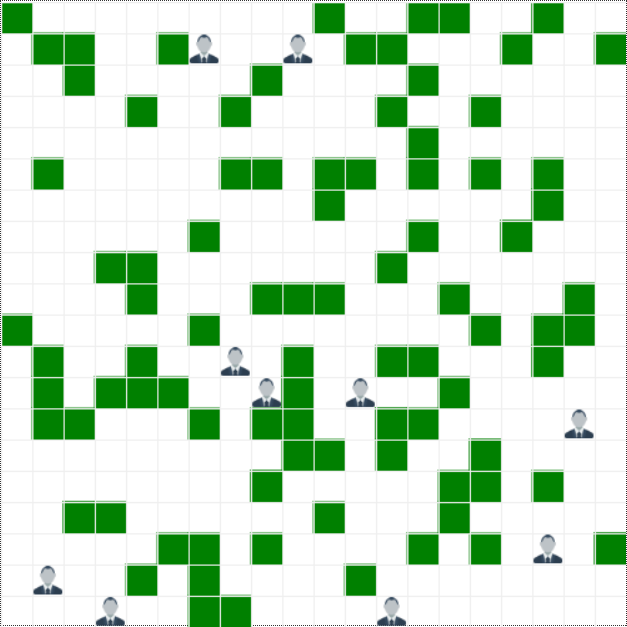
\includegraphics[width=0.48\linewidth]{images/ch03/mesa6}
	}\hfill
	\subfloat[Saat $t=84$]{
		\label{sfig:mesa7}
		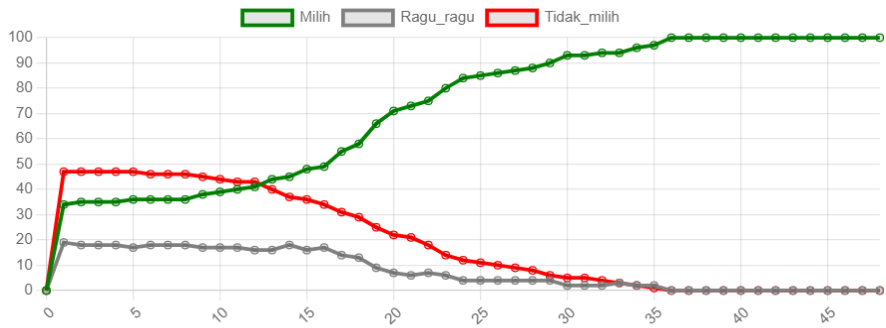
\includegraphics[width=0.48\linewidth]{images/ch03/mesa7}
	}\hfill
	\caption{Simulasi pemilihan di skenario ideal}
	\label{fig:simulasi_mesa_ideal}
\end{figure}

Seperti yang diharapkan terjadi dalam skenario ideal ini yaitu calon pemimpin dengan mudah memberikan pengaruh melalui stimulus agen bayaran agar calon pemilih mau memilih. Namun yang menjadi catatan disini adalah agen bayaran terus berada dalam sistem karena masing-masing agen masih menyimpan uang yang dapat dibagikan tapi agen pemilih sudah terpengaruh untuk ikut memilih. Sesuai dengan aturan sederhana pada sub bab \ref{sec:sbab_aturansederhana}, agen bayaran akan meninggalkan grid ketika uang sudah habis dibagikan.

\subsubsection{Skenario Optimis}

Pada skenario ini konfigurasi \texttt{input} diatur seoptimis mungkin. Hal ini dapat dilihat dalam Tabel \ref{tab:pengaturanoptimis} dibawah. Peforma calon pemimpin dianggap sempurna dalam skenario ini. Adapun sebaran acak awal untuk skenario optimis tampak pada Gambar \ref{fig:mesa8} berikut.

\begin{figure}[H]
\centering
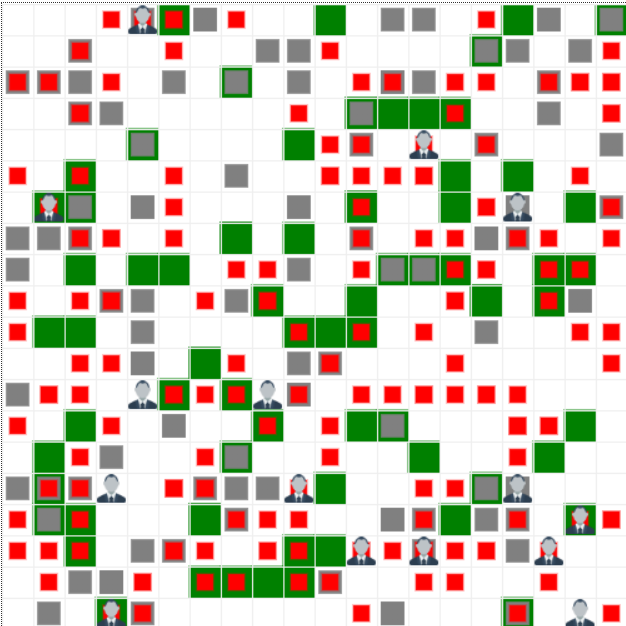
\includegraphics[width=0.8\linewidth]{images/ch03/mesa8}
\caption{Sebaran acak awal masing-masing agen}
\label{fig:mesa8}
\end{figure}


\begin{table}[H]
\centering
\caption{Pengaturan aplikasi untuk skenario ideal}
\begin{tabular}{cccccccc}
	\hline
	Peforma & $N_{ab}$ & $N_{p}$ & $Tipe_{pemilih}$ & $Tipe_{tetangga}$ & R & uang & keluar \\
	\hline
	1 & 15 & 350 & Heterogen & Moore & 4 & 1000 & 50\\
	\hline
\end{tabular}
\label{tab:pengaturanoptimis}
\end{table}

Apabila simulasi dijalankan selama 185 iterasi, tampak bahwa semua agen bayaran sudah meninggalkan sistem seperti Gambar \ref{sfig:mesa9}. Berdasarkan Gambar \ref{sfig:mesa10} pula, hal yang mengagetkan terjadi yaitu agen bayaran tidak berhasil mempengaruhi agen pemilih untuk yakin memilih secara keseluruhan. Hal ini menjadi suatu anomali karena memiliki peforma yang sempurna dengan agen bayaran yang banya serta modal yang besar tapi tetap tidak memberi pengaruh yang besar.

\begin{figure}[H]
	\centering
	\subfloat[Agen bayaran tidak aktif]{
		\label{sfig:mesa9}
		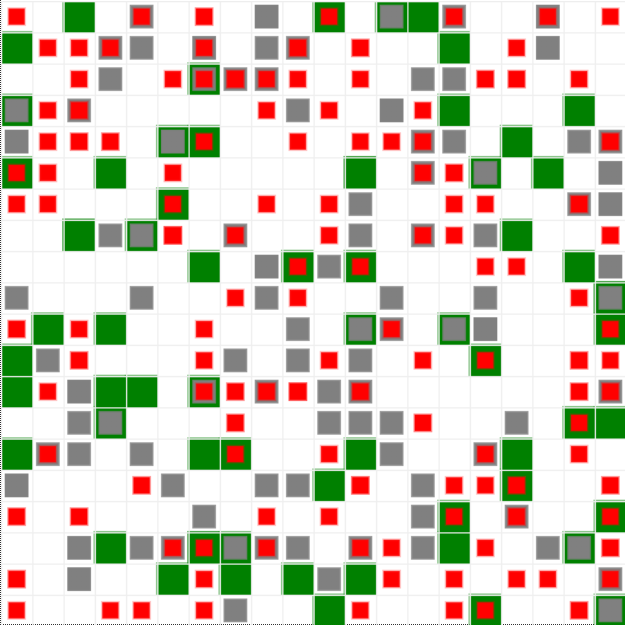
\includegraphics[width=0.48\linewidth]{images/ch03/mesa9}
	}\hfill
	\subfloat[Saat $t=185$]{
		\label{sfig:mesa10}
		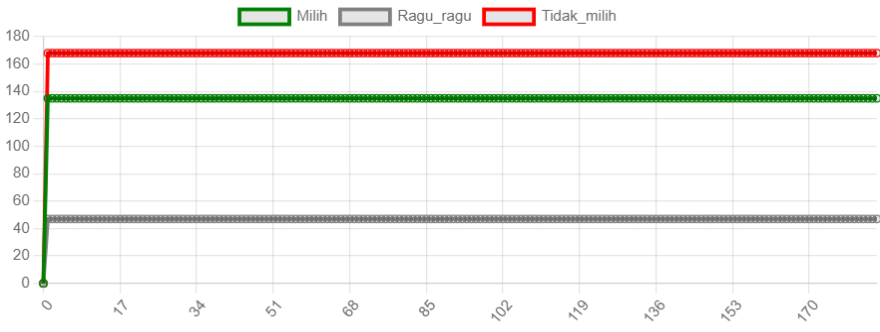
\includegraphics[width=0.48\linewidth]{images/ch03/mesa10}
	}\hfill
	\caption{Simulasi pemilihan di skenario optimis}
	\label{fig:simulasi_mesa_optimis}
\end{figure}

Apabila anomali ini dianalisis lebih lanjut lagi, penyebab yang dapat memicu fenomena ini adalah jarak radius pengamatan agen pemilih yang terlalu besar. Denga radius yang besar untuk kawasan yang dominan dengan agen pemilih yang tidak yakin memilih dapat memberikan hasil akumulasi masing-masing agen pemilih untuk tetap pada pendiriannya (tidak memilih ataupun ragu-ragu), sedangkan agen pemilih yang yakin pun kesusahan dalam memberikan pengaruh melalui interaksi agar agen lain ikut terpengaruh. Bisa saja dari faktor pengaruh dari oposisi sehingga dalam kawasan tersebut lebih dominan tidak memilih calon pemimpin tersebut.

Teknik yang dapat digunakan untuk menyiasati ini adalah dengan mengurangi jarak radius pengamatan agen pemilih sehingga dampak dari sentimen negatif dapat dihindari. Sebagai contoh dalam skenario optimis ini, radius pengamatan dikurangi menjadi $R=2$. Hasil simulasi dapat dilihat melalui Gambar \ref{sfig:mesa12}.

\begin{figure}[H]
	\centering
	\subfloat[Agen bayaran aktif]{
		\label{sfig:mesa11}
		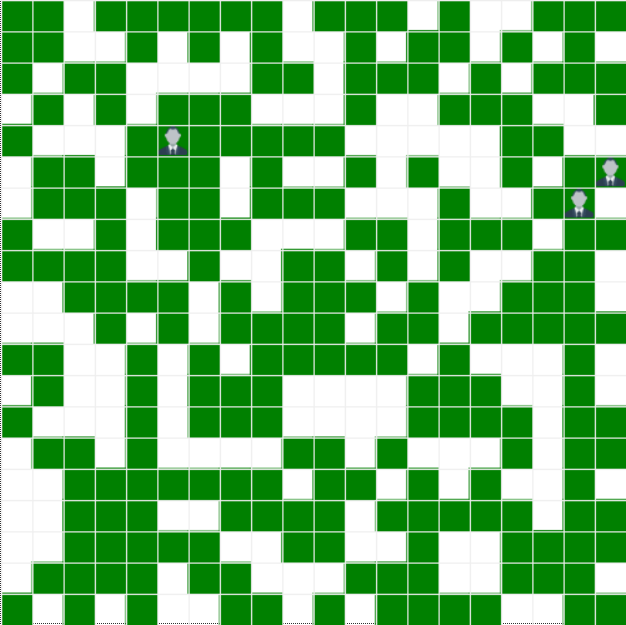
\includegraphics[width=0.48\linewidth]{images/ch03/mesa11}
	}\hfill
	\subfloat[Saat $t=119$]{
		\label{sfig:mesa12}
		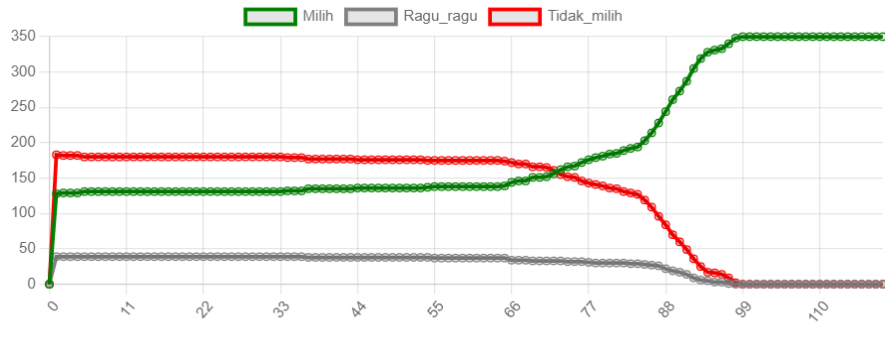
\includegraphics[width=0.48\linewidth]{images/ch03/mesa12}
	}\hfill
	\caption{Simulasi pemilihan di skenario optimis dengan pengurangan radius pengamatan}
	\label{fig:simulasi_mesa_optimis_radius}
\end{figure}

Walaupun jejaring sosial memiliki pengaruh luas sehingga dapat memberikan radius pengamatan yang besar, namun terkadang pengaruh tersebut perlu dikurangi. Cara mengurangi radius pengamatan di lapangan dapat dilakukan dengan cara menggunakan \textit{buzzer} untuk membalikkan sentimen menjadi positif. Memang dalam pemodelan yang dilakukan saat ini tidak menerapkan analisis dari pengaruh \textit{buzzer} secara langsung.
